%LTeX: language=it
\subsection{UC 12 - Modifica contatto} \label{sec:UC12}
    \begin{itemize}
        \item \textbf{Attore principale}: MUA;
        \item \textbf{Descrizione}: il MUA deve poter modificare un contatto nel sistema;
        \item \textbf{Precondizioni}: l’account che il MUA gestisce è registrato nel sistema, ha una connessione aperta con il sistema ed è autenticato;
        \item \textbf{Postcondizioni}: il contatto è stata modificato con successo, ed è stato salvato nel sistema
        \item \textbf{Scenario principale}:
            \begin{enumerate}
                \item il MUA trasmette il nuovo nome del contatto (\hyperref[sec:UC12.1]{UC 12.1});
                \item il MUA trasmette il nuovo indirizzo e-mail del contatto (\hyperref[sec:UC12.2]{UC 12.2});
                \item il sistema salva il contatto modificato;
            \end{enumerate}
        \item \textbf{Inclusioni}: nessuna;
        \item \textbf{Generalizzazioni}: nessuna;
        \item \textbf{Estensioni}: nessuna.
    \end{itemize}

\begin{figure}[h]
    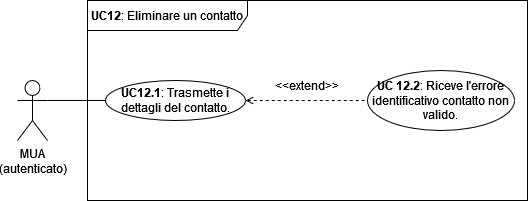
\includegraphics[width=0.85\textwidth]{sections/uc_imgs/UC12.png}
    \centering
    \caption{Diagramma sotto-casi UC 12}
\end{figure}

\subsubsection{UC 12.1 - Trasmette nome contatto} \label{sec:UC12.1}
    \begin{itemize}
        \item \textbf{Attore principale}: MUA;
        \item \textbf{Descrizione}: il MUA trasmette il nuovo nome per modificare il contatto al sistema;
        \item \textbf{Precondizioni}: il MUA sta usando la funzionalità di modifica di un contatto;
        \item \textbf{Postcondizioni}: il sistema conosce il nuovo nome del contatto;
        \item \textbf{Scenario principale}:
            \begin{enumerate}
                \item il MUA invia il nuovo nome per modificare il contatto al sistema;
                \item il sistema controlla che le informazioni ricevute rispettino il seguente requisito minimo:
                    \begin{itemize}
                        \item il nome del contatto non è una stringa vuota;
                    \end{itemize}
            \end{enumerate}
        \item \textbf{Inclusioni}: nessuna;
        \item \textbf{Generalizzazioni}: nessuna;
        \item \textbf{Estensioni}:
            \begin{enumerate}[label=\alph*.]
                \item il sistema non riesce a modificare il contatto perché il nome fornito non è valido:
                \begin{enumerate}[label=\arabic*.]
                    \item il sistema ritorna un errore al MUA di nome non valido (\hyperref[sec:UC12.3]{UC 12.3}).
                \end{enumerate}
            \end{enumerate}
    \end{itemize}


    \subsubsection{UC 12.2 - Trasmette l'indirizzo e-mail del contatto} \label{sec:UC12.2}
    \begin{itemize}
        \item \textbf{Attore principale}: MUA;
        \item \textbf{Descrizione}: il MUA trasmette il nuovo indirizzo e-mail per modificare il contatto al sistema;
        \item \textbf{Precondizioni}: il MUA sta usando la funzionalità di modifica di un contatto;
        \item \textbf{Postcondizioni}: il sistema conosce il nuovo indirizzo e-mail del contatto;
        \item \textbf{Scenario principale}:
            \begin{enumerate}
                \item il MUA invia il nuovo indirizzo e-mail per modificare il contatto al sistema;
                \item il sistema controlla che le informazioni ricevute rispettino il seguente requisito minimo:
                    \begin{itemize}
                        \item l'indirizzo e-mail del contatto non è una stringa vuota;
                    \end{itemize}
            \end{enumerate}
        \item \textbf{Inclusioni}: nessuna;
        \item \textbf{Generalizzazioni}: nessuna;
        \item \textbf{Estensioni}:
            \begin{enumerate}[label=\alph*.]
                \item il sistema non riesce a modificare il contatto perché l'indirizzo e-mail fornito non è valido:
                \begin{enumerate}[label=\arabic*.]
                    \item il sistema ritorna un errore al MUA di indirizzo e-mail non valido (\hyperref[sec:UC12.4]{UC 12.4}).
                \end{enumerate}
            \end{enumerate}
    \end{itemize}


\subsubsection{UC 12.3 - Ritorna l'errore nome non valido} \label{sec:UC12.3}
    \begin{itemize}
        \item \textbf{Attore principale}: MUA;
        \item \textbf{Descrizione}: il sistema non riesce a modificare il contatto perché il nome del contatto non rispetta i requisiti;
        \item \textbf{Precondizioni}: il MUA ha inviato il nome del contatto;
        \item \textbf{Postcondizioni}: il sistema non modifica il contatto, il MUA è stato notificato dell'errore;
        \item \textbf{Scenario principale}:
            \begin{enumerate}
                \item il sistema controlla la sintassi del nome del contatto e trova un errore;
                \item il sistema non modifica il contatto e notifica il MUA dell'errore;
            \end{enumerate}
        \item \textbf{Inclusioni}: nessuna;
        \item \textbf{Generalizzazioni}: nessuna;
        \item \textbf{Estensioni}: nessuna.
    \end{itemize}

\subsubsection{UC 12.4 - Ritorna l'errore indirizzo e-mail non valido} \label{sec:UC12.4}
    \begin{itemize}
        \item \textbf{Attore principale}: MUA;
        \item \textbf{Descrizione}: il sistema non riesce a modificare il contatto perché l'indirizzo e-mail del contatto non rispetta i requisiti;
        \item \textbf{Precondizioni}: il MUA ha inviato l'indirizzo e-mail del contatto;
        \item \textbf{Postcondizioni}: il sistema non modifica il contatto, il MUA è stato notificato dell'errore;
        \item \textbf{Scenario principale}:
            \begin{enumerate}
                \item il sistema controlla la sintassi dell'indirizzo e-mail del contatto e trova un errore;
                \item il sistema non modifica il contatto e notifica il MUA dell'errore;
            \end{enumerate}
        \item \textbf{Inclusioni}: nessuna;
        \item \textbf{Generalizzazioni}: nessuna;
        \item \textbf{Estensioni}: nessuna.
    \end{itemize}